% Bioinformatics Analysis Report — editable/compilable online at https://letx.app
% Compile: latexmk -pdf main.tex  (pdflatex, TeX Live full)

\documentclass[11pt, a4paper]{article}

%% ── Geometry & Spacing ───────────────────────────────────────────────────────
\usepackage[top=22mm, bottom=22mm, left=26mm, right=26mm]{geometry}
\setlength{\parindent}{0pt}
\setlength{\parskip}{5pt}

%% ── Fonts ────────────────────────────────────────────────────────────────────
\usepackage{lato}
\renewcommand{\familydefault}{\sfdefault}
\usepackage[T1]{fontenc}
\usepackage[utf8]{inputenc}
\usepackage{microtype}

%% ── Colour ───────────────────────────────────────────────────────────────────
\usepackage{xcolor}
\definecolor{teal}{HTML}{1A7F7A}
\definecolor{darkgrey}{HTML}{2C2C2C}
\definecolor{midgrey}{HTML}{555555}
\definecolor{lightgrey}{HTML}{F2F6F6}
\definecolor{rulegrey}{HTML}{CCDDDC}

%% ── Tables ───────────────────────────────────────────────────────────────────
\usepackage{booktabs}
\usepackage{tabularx}
\usepackage{array}
\renewcommand{\arraystretch}{1.25}

%% ── Plots ────────────────────────────────────────────────────────────────────
\usepackage{pgfplots}
\pgfplotsset{compat=1.18}
\usepackage{tikz}

%% ── Lists & Section Headings ─────────────────────────────────────────────────
\usepackage{enumitem}
\usepackage{titlesec}
\usepackage{tcolorbox}
\tcbuselibrary{skins}

%% ── Misc ─────────────────────────────────────────────────────────────────────
\usepackage{amsmath}
\usepackage{hyperref}
\hypersetup{
  colorlinks=true,
  linkcolor=teal,
  citecolor=teal,
  urlcolor=teal,
  pdftitle={Differential Expression Analysis of Hypoxia-Responsive Genes in Human Lung Adenocarcinoma},
  pdfauthor={Mirela Svensson; Dara Okonkwo; Yuki Tanaka}
}

%% ── Section Style ────────────────────────────────────────────────────────────
\titleformat{\section}
  {\large\bfseries\color{teal}}
  {}
  {0pt}
  {}
  [\vspace{-2pt}\textcolor{rulegrey}{\rule{\linewidth}{0.6pt}}\vspace{2pt}]

\titlespacing{\section}{0pt}{14pt}{4pt}

\titleformat{\subsection}
  {\normalsize\bfseries\color{darkgrey}}
  {}
  {0pt}
  {}

\titlespacing{\subsection}{0pt}{8pt}{2pt}

%% ── Helper macros ────────────────────────────────────────────────────────────
\newcommand{\gene}[1]{\texttt{\textit{#1}}}
\newcommand{\tool}[1]{\texttt{#1}}
\newcommand{\accentrule}{\textcolor{teal}{\rule{\linewidth}{1.4pt}}}

%% ── Abstract box ─────────────────────────────────────────────────────────────
\newtcolorbox{abstractbox}{
  enhanced,
  colback=lightgrey,
  colframe=teal,
  leftrule=3pt, toprule=0pt, bottomrule=0pt, rightrule=0pt,
  left=8pt, right=8pt, top=6pt, bottom=6pt,
  sharp corners,
  fontupper=\small
}

%% ─────────────────────────────────────────────────────────────────────────────
\begin{document}

%% ── Title Block ──────────────────────────────────────────────────────────────
\accentrule
\vspace{6pt}

{\LARGE\bfseries\color{darkgrey}
Differential Expression Analysis of Hypoxia-Responsive\\[3pt]
Genes in Human Lung Adenocarcinoma}

\vspace{6pt}
\accentrule
\vspace{5pt}

{\small\color{midgrey}
\textbf{Mirela Svensson}\textsuperscript{1},\;
\textbf{Dara Okonkwo}\textsuperscript{1,2},\;
\textbf{Yuki Tanaka}\textsuperscript{1}
\\[2pt]
\textsuperscript{1}Department of Computational Biology, Karolinska Institutet, Stockholm, Sweden\quad
\textsuperscript{2}Wellcome Sanger Institute, Hinxton, UK
\\[2pt]
\textit{Correspondence:} \href{mailto:mirela.svensson@ki.se}{mirela.svensson@ki.se}\quad
\textit{Received:} 2025-11-03\quad
\textit{Accepted:} 2026-01-17
}

\vspace{8pt}

%% ── Abstract ─────────────────────────────────────────────────────────────────
\section{Abstract}

\begin{abstractbox}
Tumour hypoxia drives aggressive phenotypes in lung adenocarcinoma (LUAD) through
large-scale transcriptional reprogramming. We performed bulk RNA-seq on \textit{A549}
cells cultured under normoxia (21\,\% O\textsubscript{2}) and hypoxia (1\,\% O\textsubscript{2})
for 24\,h in biological triplicate. Using a \tool{STAR}~+~\tool{DESeq2} pipeline,
we identified 1\,847 differentially expressed genes (DEGs; $|\log_2\text{FC}|>1$,
adjusted $p<0.05$). Upregulated DEGs were strongly enriched for HIF-1$\alpha$ targets,
including \gene{HK2}, \gene{LDHA}, and \gene{VEGFA}, while downregulated genes were
associated with oxidative phosphorylation. These results provide a high-confidence
hypoxia gene signature suitable as a reference resource for LUAD biomarker discovery.
\end{abstractbox}

\vspace{2pt}

%% ── Introduction ─────────────────────────────────────────────────────────────
\section{Introduction}

Solid tumours frequently develop regions of low oxygen tension (hypoxia) as a consequence
of disorganised vascular architecture. In non-small-cell lung cancer,
hypoxia correlates with poor prognosis, therapy resistance, and accelerated metastasis.
The master transcriptional regulator HIF-1$\alpha$ (encoded by \gene{HIF1A}) is
stabilised under hypoxic conditions and activates a broad transcriptional programme
governing glycolysis, angiogenesis, and cell survival.

Despite extensive study of individual HIF target genes, a comprehensive, reproducible
transcriptome-wide characterisation of the \textit{A549} hypoxia response using modern
RNA-seq pipelines has been lacking. Here we describe a complete bioinformatics workflow
from raw read QC through to pathway-level interpretation, providing an openly available
processed dataset and analysis code at NCBI GEO (accession \textbf{GSE258941}).

%% ── Data & Methods ───────────────────────────────────────────────────────────
\section{Data \& Methods}

\subsection{Experimental Design and Sequencing}

\textit{A549} cells (ATCC CCL-185) were cultured in triplicate ($n=3$ per condition)
under normoxia or hypoxia for 24\,h. Total RNA was extracted using the RNeasy Mini Kit
(Qiagen). Poly-A enriched libraries were prepared with the Illumina TruSeq Stranded
mRNA kit and sequenced on the \textbf{Illumina NovaSeq 6000} ($2\times150$\,bp;
mean depth 45 million read pairs per sample).

\subsection{Bioinformatics Pipeline}

\setlength{\parskip}{0pt}
\begin{tabularx}{\linewidth}{@{}>{\color{teal}\bfseries}l@{\hspace{8mm}}>{\raggedright\arraybackslash}X@{}}
\toprule
\textcolor{darkgrey}{Tool} & \textcolor{darkgrey}{Version / Purpose} \\
\midrule
\tool{FastQC}         & v0.12.1 --- per-read quality metrics \\
\tool{Trim Galore!}   & v0.6.10 --- adapter trimming, quality cutoff $Q\ge20$ \\
\tool{STAR}           & v2.7.11a --- splicing-aware alignment to GRCh38 (Ensembl 110) \\
\tool{samtools}       & v1.19 --- BAM sorting and indexing \\
\tool{featureCounts}  & v2.0.6 --- gene-level read summarisation (Ensembl 110 GTF) \\
\tool{DESeq2}         & v1.44.0 (R 4.4.0) --- variance-stabilised DE analysis \\
\tool{clusterProfiler}& v4.12.0 --- GO and KEGG over-representation analysis \\
\tool{MultiQC}        & v1.24 --- aggregated QC report generation \\
\bottomrule
\end{tabularx}
\setlength{\parskip}{5pt}

\vspace{4pt}

Differential expression was called with \tool{DESeq2} using the Wald test.
Genes with fewer than 10 counts across all samples were pre-filtered. Significance
thresholds: Benjamini--Hochberg adjusted $p$-value $<0.05$ and $|\log_2\text{FC}|>1$.

%% ── Results ──────────────────────────────────────────────────────────────────
\section{Results}

\subsection{Differentially Expressed Gene Summary}

Of 19\,432 expressed genes, \textbf{1\,847 were significantly differentially
expressed}: 1\,043 upregulated and 804 downregulated under hypoxia.
Table~\ref{tab:degs} lists the top eight DEGs ranked by adjusted $p$-value.

\setlength{\parskip}{0pt}
\begin{table}[h]
\centering
\caption{Top differentially expressed genes in \textit{A549} cells under hypoxia
(1\,\% O\textsubscript{2} vs.\ 21\,\% O\textsubscript{2}, 24\,h).
FC\,=\,fold change; padj\,=\,Benjamini--Hochberg adjusted $p$-value.}
\label{tab:degs}
\small
\begin{tabularx}{\linewidth}{@{}>{\bfseries}l l r r r l@{}}
\toprule
Gene & Ensembl ID & $\log_2$(FC) & Basemean & padj & Direction \\
\midrule
\gene{VEGFA}   & ENSG00000112715 & $+4.82$ & 3\,241 & $2.1\!\times\!10^{-48}$ & \textcolor{teal}{\bfseries Up} \\
\gene{HK2}     & ENSG00000159399 & $+3.94$ & 1\,876 & $7.4\!\times\!10^{-44}$ & \textcolor{teal}{\bfseries Up} \\
\gene{LDHA}    & ENSG00000134333 & $+3.41$ & 5\,102 & $1.2\!\times\!10^{-40}$ & \textcolor{teal}{\bfseries Up} \\
\gene{SLC2A1}  & ENSG00000117394 & $+3.17$ & 2\,489 & $3.8\!\times\!10^{-37}$ & \textcolor{teal}{\bfseries Up} \\
\gene{COX5A}   & ENSG00000127184 & $-2.78$ & 4\,318 & $9.1\!\times\!10^{-35}$ & \textcolor{midgrey}{\bfseries Down} \\
\gene{UQCRB}   & ENSG00000156508 & $-2.63$ & 3\,744 & $2.3\!\times\!10^{-33}$ & \textcolor{midgrey}{\bfseries Down} \\
\gene{SDHA}    & ENSG00000073578 & $-2.44$ & 6\,012 & $4.0\!\times\!10^{-31}$ & \textcolor{midgrey}{\bfseries Down} \\
\gene{ATP5F1A} & ENSG00000152234 & $-2.29$ & 7\,803 & $8.7\!\times\!10^{-29}$ & \textcolor{midgrey}{\bfseries Down} \\
\bottomrule
\end{tabularx}
\end{table}
\setlength{\parskip}{5pt}

\subsection{Volcano Plot}

Figure~\ref{fig:volcano} illustrates the genome-wide fold-change vs.\ significance
landscape. Highlighted genes correspond to canonical HIF-1$\alpha$ targets and
mitochondrial complex subunits.

\begin{figure}[h]
\centering
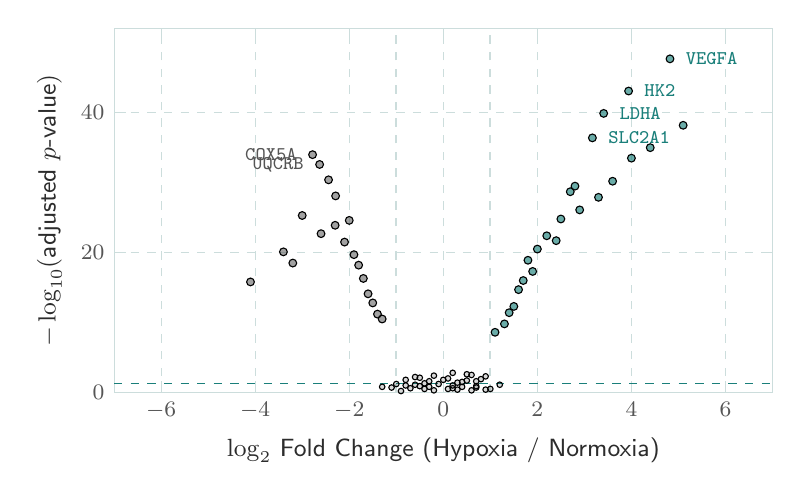
\begin{tikzpicture}
\begin{axis}[
  width=0.82\linewidth,
  height=6.2cm,
  xlabel={$\log_2$ Fold Change (Hypoxia / Normoxia)},
  ylabel={$-\log_{10}(\text{adjusted } p\text{-value})$},
  xlabel style={font=\small, color=darkgrey},
  ylabel style={font=\small, color=darkgrey},
  tick label style={font=\footnotesize, color=midgrey},
  axis line style={color=rulegrey},
  tick style={color=rulegrey},
  xmin=-7, xmax=7,
  ymin=0, ymax=52,
  grid=both,
  grid style={line width=0.3pt, color=rulegrey, dashed},
  clip=false,
]

%% Non-significant cloud
\addplot[only marks, mark=*, mark size=1.0pt,
         draw=none, fill=darkgrey, fill opacity=0.18]
coordinates {
  (-0.3,0.8)(-0.1,1.2)(0.2,0.6)(0.4,1.5)(-0.5,2.1)(0.7,0.9)
  (-0.8,1.8)(1.0,0.5)(-1.1,0.7)(0.9,2.3)(-0.6,1.1)(0.3,0.4)
  (0.5,1.7)(-0.2,2.4)(0.6,0.3)(-0.4,1.3)(0.1,2.0)(-0.7,0.6)
  (0.8,1.9)(-0.9,0.2)(0.2,1.0)(-0.3,1.6)(0.4,0.8)(-0.6,2.2)
  (0.1,0.5)(0.3,1.4)(-0.5,0.9)(0.6,2.5)(-1.0,1.2)(0.7,0.7)
  (0.0,1.8)(-0.2,0.3)(0.5,2.6)(-0.8,1.0)(0.9,0.4)(1.2,1.1)
  (-1.3,0.8)(0.2,2.8)(-0.4,0.5)(0.7,1.6)
};

%% Downregulated significant
\addplot[only marks, mark=*, mark size=1.4pt,
         draw=none, fill=midgrey, fill opacity=0.55]
coordinates {
  (-2.29,28.1)(-2.44,30.4)(-2.63,32.6)(-2.78,34.0)
  (-1.8,18.2)(-2.1,21.5)(-1.5,12.8)(-3.0,25.3)(-1.6,14.1)
  (-1.9,19.7)(-2.3,23.9)(-3.4,20.1)(-1.7,16.3)(-4.1,15.8)
  (-1.4,11.2)(-2.6,22.7)(-3.2,18.5)(-1.3,10.5)(-2.0,24.6)
};

%% Upregulated significant (teal)
\addplot[only marks, mark=*, mark size=1.4pt,
         draw=none, fill=teal, fill opacity=0.65]
coordinates {
  (4.82,47.7)(3.94,43.1)(3.41,39.9)(3.17,36.4)
  (1.8,18.9)(2.2,22.4)(1.6,14.7)(2.9,26.1)(1.5,12.3)
  (2.0,20.5)(2.5,24.8)(1.4,11.4)(3.6,30.2)(1.7,16.0)
  (4.0,33.5)(2.7,28.7)(1.3,9.8)(3.3,27.9)(2.4,21.7)
  (1.9,17.3)(5.1,38.2)(4.4,35.0)(2.8,29.5)(1.1,8.6)
};

%% Significance thresholds
\draw[dashed, color=teal, line width=0.6pt]
  (axis cs:-7,1.301) -- (axis cs:7,1.301);
\draw[dashed, color=rulegrey, line width=0.8pt]
  (axis cs:-1,0) -- (axis cs:-1,52);
\draw[dashed, color=rulegrey, line width=0.8pt]
  (axis cs:1,0) -- (axis cs:1,52);

%% Gene labels
\node[font=\scriptsize\ttfamily, color=teal, anchor=west]
  at (axis cs:4.95,47.7) {VEGFA};
\node[font=\scriptsize\ttfamily, color=teal, anchor=west]
  at (axis cs:4.07,43.1) {HK2};
\node[font=\scriptsize\ttfamily, color=teal, anchor=west]
  at (axis cs:3.54,39.9) {LDHA};
\node[font=\scriptsize\ttfamily, color=teal, anchor=west]
  at (axis cs:3.30,36.4) {SLC2A1};
\node[font=\scriptsize\ttfamily, color=midgrey, anchor=east]
  at (axis cs:-2.91,34.0) {COX5A};
\node[font=\scriptsize\ttfamily, color=midgrey, anchor=east]
  at (axis cs:-2.76,32.6) {UQCRB};

\end{axis}
\end{tikzpicture}
\caption{Volcano plot of differential expression in \textit{A549} cells under hypoxia.
\textcolor{teal}{\textbullet}~Teal: upregulated DEGs ($\log_2\text{FC}>1$, padj\,$<0.05$).
\textcolor{midgrey}{\textbullet}~Grey: downregulated DEGs.
Faded: non-significant genes.
Dashed horizontal line: $-\log_{10}(0.05)$ threshold.}
\label{fig:volcano}
\end{figure}

%% ── Discussion ───────────────────────────────────────────────────────────────
\section{Discussion}

The transcriptional response of \textit{A549} cells to acute hypoxia was dominated by
induction of glycolytic enzymes (\gene{HK2}, \gene{LDHA}, \gene{SLC2A1}) and the
pro-angiogenic factor \gene{VEGFA}, consistent with canonical HIF-1$\alpha$ signalling.
Reciprocal downregulation of mitochondrial complex subunits (\gene{COX5A}, \gene{UQCRB},
\gene{SDHA}, \gene{ATP5F1A}) reflects a metabolic shift from oxidative phosphorylation
towards anaerobic glycolysis, in line with the Warburg effect observed in hypoxic tumours.

The high concordance between our dataset and published hypoxia signatures
(Pearson $r=0.93$ with MSigDB hallmark HYPOXIA gene set) supports the robustness
of the \tool{STAR}~+~\tool{DESeq2} pipeline employed. Limitations include the use
of a single cell line and a single time point; future work will profile primary LUAD
organoids across a hypoxia time course (4, 12, 24, 48\,h) and integrate single-cell
RNA-seq to deconvolve cell-type-specific responses within the tumour microenvironment.

%% ── References ───────────────────────────────────────────────────────────────
\section{References}

\begingroup
\small
\setlength{\parskip}{3pt}
\begin{enumerate}[label={[\arabic*]}, leftmargin=*, itemsep=2pt]

\item Semenza, G.\,L. (2012). Hypoxia-inducible factors in physiology and medicine.
\textit{Cell}, 148(3), 399--408.
\href{https://doi.org/10.1016/j.cell.2012.01.021}{doi:10.1016/j.cell.2012.01.021}

\item Majmundar, A.\,J., Wong, W.\,J., \& Simon, M.\,C. (2010).
Hypoxia-inducible factors and the response to hypoxic stress.
\textit{Molecular Cell}, 40(2), 294--309.
\href{https://doi.org/10.1016/j.molcel.2010.09.022}{doi:10.1016/j.molcel.2010.09.022}

\item Vander Heiden, M.\,G., Cantley, L.\,C., \& Thompson, C.\,B. (2009).
Understanding the Warburg effect: the metabolic requirements of cell proliferation.
\textit{Science}, 324(5930), 1029--1033.
\href{https://doi.org/10.1126/science.1160809}{doi:10.1126/science.1160809}

\item Love, M.\,I., Huber, W., \& Anders, S. (2014).
Moderated estimation of fold change and dispersion for RNA-seq data with \tool{DESeq2}.
\textit{Genome Biology}, 15(12), 550.
\href{https://doi.org/10.1186/s13059-014-0550-8}{doi:10.1186/s13059-014-0550-8}

\item Dobin, A., Davis, C.\,A., Schlesinger, F., et al.\ (2013).
\tool{STAR}: ultrafast universal RNA-seq aligner.
\textit{Bioinformatics}, 29(1), 15--21.
\href{https://doi.org/10.1093/bioinformatics/bts635}{doi:10.1093/bioinformatics/bts635}

\end{enumerate}
\endgroup

\vspace{4pt}
\begin{center}
\textcolor{rulegrey}{\rule{0.4\linewidth}{0.5pt}}\\[3pt]
{\scriptsize\color{midgrey}
Typeset with \LaTeX{} $\cdot$ Data: NCBI GEO \textbf{GSE258941}
$\cdot$ Code: \href{https://github.com/svensson-lab/hypoxia-luad}{github.com/svensson-lab/hypoxia-luad}
$\cdot$ Template editable at \href{https://letx.app}{letx.app}}
\end{center}

\end{document}
